\section{UMA task definition and feature dictionary}
\label{app:prediction}

The task contains 810 retrospectively eligible requests, of which 466 resolve to a value different from the proposal and 344 retain the proposed value. A changed value is an institutional adjudication label. The cohort is restricted to challenged, linked and reconciled requests, so these proportions do not estimate the prevalence of incorrect proposals in the full request population.

Excluding early expiration leaves 413 requests with 69 changed proposals; restricting resolutions to binary zero or one leaves 402 requests with 59 changes. These cohorts support sensitivity analysis. The main task keeps native classes because early expiration differs from either binary outcome.
\begin{figure}[!htbp]
\centering
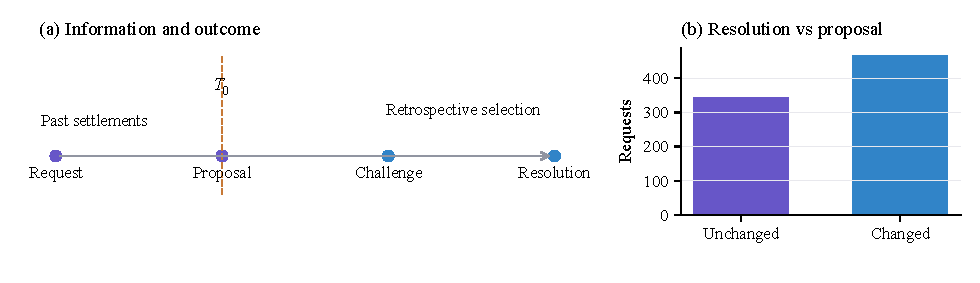
\includegraphics[width=0.99\linewidth]{figures/prediction_task.pdf}
\caption{Information boundary and target of the UMA task. (a) $T_0$ is the proposal event; prior-history features use earlier settled requests. Challenge and resolution determine retrospective eligibility and the outcome. (b) Counts compare the native proposed and resolved integers, retaining special resolution classes.}
\label{fig:prediction_task}
\end{figure}

Let $B$, $F$ and $R$ denote the effective bond, final fee and configured reward in the asset's smallest units. For address $a$ in a specified role, $N_a$ counts retained prior settlements, $D_a$ counts those challenged, and $J_a$ counts those whose challenged proposal was rejected. Prior settlements must precede the proposal in block, transaction and log order. Proposer and requester histories are separate and bounded by the retained records.

\begin{table}[!htbp]
\centering\tabstyle
\caption{Sixteen candidate features. Rates with $N_a=0$ and ratios with $B=0$ are missing. Parameter-derived entries require historical binding before they can be certified as available at the proposal.}
\label{tab:prediction_features}
\begin{tabularx}{\linewidth}{@{}L{.30\linewidth}L{.24\linewidth}Y@{}}
\toprule Feature & Definition or unit & Evidence / missingness \\ \midrule
Bond magnitude & $\log(1+B)$ & Reconstructed effective bond; historical parameter binding. \\
Final-fee magnitude & $\log(1+F)$ & Native fee; missing if absent. \\
Reward magnitude & $\log(1+R)$ & Configured adapter reward; historical binding. \\
Reward--bond ratio & $R/B$ & Same-asset amounts; undefined for zero bond. \\
Liveness & Expiry minus proposal, hours & Proposal event and recorded expiry. \\
Proposal latency & Proposal minus request event, hours & Execution clocks, not request-reference time. \\
Ancillary length & Decoded byte count & Native request payload. \\
Proposer prior count & $N_a$ & Earlier settlements in proposer role. \\
Proposer dispute rate & $D_a/N_a$ & Missing when no prior settlement is retained. \\
Proposer rejection rate & $J_a/N_a$ & Rejected challenged proposals among prior settlements. \\
Requester prior count & $N_a$ & Earlier settlements in requester role. \\
Requester dispute rate & $D_a/N_a$ & Missing when no prior settlement is retained. \\
Requester rejection rate & $J_a/N_a$ & Same-role prior settlement outcomes. \\
Registered adapter & Binary membership & Requester contract registry. \\
Proposed price class & Zero, one, half, early expiry, other & Native proposed integer; no forced binary recoding. \\
Adapter version & Registered implementation class & Historical source binding required. \\
\bottomrule
\end{tabularx}
\end{table}

Feature availability is recorded for each request and feature. Native event fields, reconstructed past histories and parameters requiring historical binding have distinct statuses. Fields used only to establish the eventual label remain outside the feature allowlist. Missing rates are retained as missing values so that subsequent users can choose and document their own preprocessing. Figure~\ref{fig:prediction_features} presents the feature distributions; no predictive model is fitted as part of this data description.
\begin{figure}[!htbp]
\centering
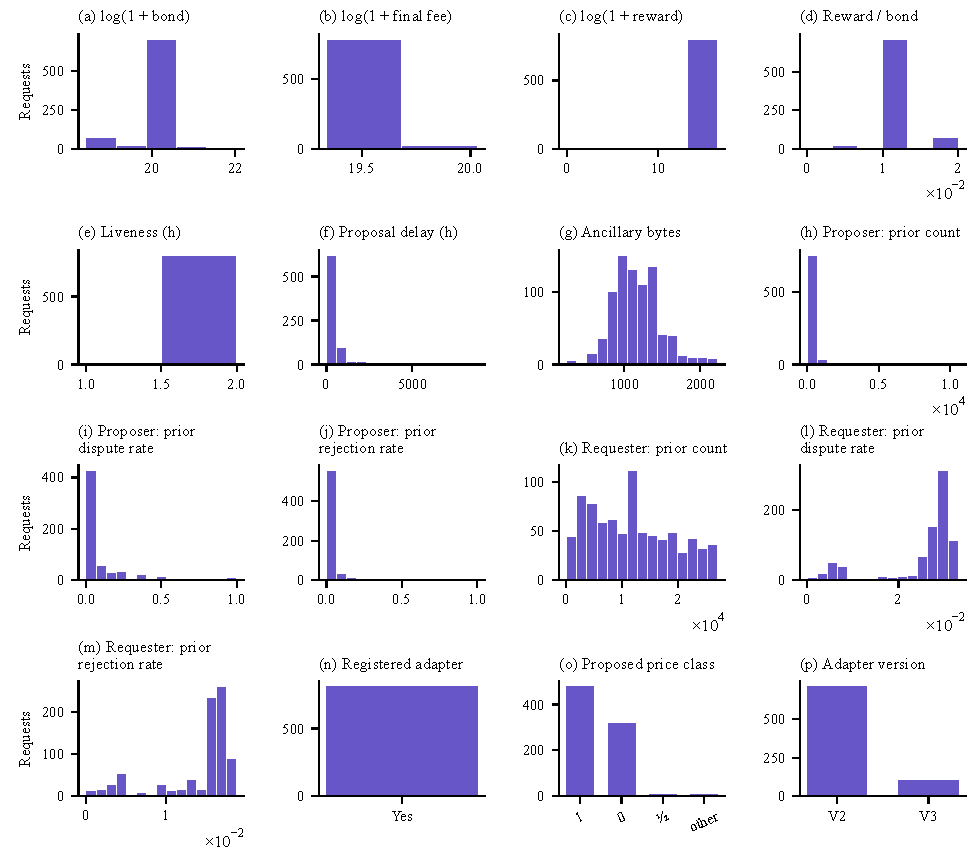
\includegraphics[width=0.99\linewidth]{figures/prediction_features.pdf}
\caption{Distributions of the sixteen task features. Histograms use nonmissing observations on the units in Table~\ref{tab:prediction_features}; categorical panels retain the recorded classes. Prior-history rates exclude requests with no retained earlier settlement in that role. Detailed missingness and availability statuses accompany the task data.}
\label{fig:prediction_features}
\end{figure}
